\documentclass{beamer}
\usepackage[utf8]{inputenc}
\usepackage[spanish]{babel}
\usepackage{graphicx}
\usepackage{booktabs}
\usepackage{amsmath}
\usepackage{listings}
\usepackage{xcolor}

\usetheme{Madrid}
\usecolortheme{default}

% Configuración de colores para bloques de código
\definecolor{codegreen}{rgb}{0,0.6,0}
\definecolor{codegray}{rgb}{0.5,0.5,0.5}
\definecolor{codepurple}{rgb}{0.58,0,0.82}
\definecolor{backcolour}{rgb}{0.95,0.95,0.92}

\lstdefinestyle{pythonstyle}{
    backgroundcolor=\color{backcolour},   
    commentstyle=\color{codegreen},
    keywordstyle=\color{blue},
    stringstyle=\color{codepurple},
    basicstyle=\ttfamily\scriptsize,
    breaklines=true,                 
    keepspaces=true,                 
    numbers=none,
    showspaces=false,                
    showstringspaces=false,
}
\lstset{style=pythonstyle, language=Python}

\title[Regresión Lineal]{Módulo 4: Aprendizaje Automático}
\subtitle{Clase 3: Regresión Lineal Simple y Múltiple}
\author{Diplomado en Ciencia de Datos}
\date{\today}

\begin{document}

\frame{\titlepage}

% -------------------------
% SECCIÓN 1: INTRODUCCIÓN
% -------------------------
\begin{frame}
\frametitle{¿Qué es la Regresión Lineal?}
\begin{block}{Definición}
Es un algoritmo fundamental de Aprendizaje Supervisado utilizado para predecir o estimar un valor numérico continuo (como precios, temperatura o ventas), basándose en la relación matemática entre distintas variables.
\end{block}
\vspace{0.3cm}
\textbf{Nuestro Caso de Estudio: Seguros Médicos}\\
Deseamos estimar el costo anual del seguro médico de un paciente. ¿De qué factores estadísticos depende esta estimación?
\begin{itemize}
    \item \textbf{Edad:} Variable Numérica Continua.
    \item \textbf{Índice de Masa Corporal (IMC):} Variable Numérica Continua.
    \item \textbf{Condición de Fumador:} Variable Categórica.
\end{itemize}
\end{frame}

% -------------------------
% SECCIÓN 2: PREPROCESAMIENTO
% -------------------------
\begin{frame}
\frametitle{Paso 1: Preprocesamiento de Datos}
Antes de aplicar cualquier modelo de regresión, la matriz de datos debe estar estructurada matemáticamente. Recordando la Sesión 2, aplicaremos tres procesos críticos:
\vspace{0.3cm}
\begin{enumerate}
    \item \textbf{Imputación de Valores Nulos:} Reemplazo de datos faltantes.
    \item \textbf{Codificación Categórica (One-Hot Encoding):} Transformación de texto a binario.
    \item \textbf{Escalado de Magnitudes:} Estandarización de variables numéricas.
\end{enumerate}
\end{frame}

\begin{frame}[fragile]
\frametitle{Comandos en Pandas: Imputación y Codificación}
En nuestro cuaderno de trabajo (Jupyter Notebook), utilizaremos los siguientes comandos de la librería \texttt{pandas}:

\begin{block}{1. Imputación mediante Mediana}
\begin{lstlisting}
mediana_bmi = df_seguros['bmi'].median()
df_seguros['bmi'] = df_seguros['bmi'].fillna(mediana_bmi)
\end{lstlisting}
El método \texttt{fillna()} busca cualquier valor \texttt{NaN} en la columna y lo reemplaza por el valor estadístico de la mediana.
\end{block}

\begin{block}{2. One-Hot Encoding}
\begin{lstlisting}
df_final = pd.get_dummies(df_seguros, columns=['sex', 'smoker'], drop_first=True)
\end{lstlisting}
El comando \texttt{get\_dummies()} convierte variables categóricas en columnas binarias (0 y 1). El parámetro \texttt{drop\_first=True} es esencial en regresión lineal para evitar la redundancia matemática (colinealidad perfecta).
\end{block}
\end{frame}

% -------------------------
% SECCIÓN 3: CORRELACIÓN
% -------------------------
\begin{frame}
\frametitle{Análisis Exploratorio: Correlación}
La regresión asume que existe una \textbf{relación lineal} entre la variable independiente ($X$) y la objetivo ($y$). 

Para verificar esto, utilizamos el \textbf{Coeficiente de Correlación de Pearson ($r$)}.
\begin{itemize}
    \item $r = 1.0$: Relación positiva perfecta.
    \item $r = -1.0$: Relación negativa perfecta.
    \item $r = 0.0$: Ausencia de correlación lineal.
\end{itemize}
\end{frame}

\begin{frame}[fragile]
\frametitle{Comandos: Visualización de Dispersión y Correlación}
Podemos verificar la correlación tanto matemática como visualmente:

\begin{block}{Gráfico de Dispersión (Scatter Plot)}
\begin{lstlisting}
import seaborn as sns
import matplotlib.pyplot as plt

sns.scatterplot(data=df_final, x='age', y='charges')
plt.show()
\end{lstlisting}
Esto genera un plano cartesiano donde cada punto es un paciente. El eje X representa la edad y el eje Y los cargos.
\end{block}

\begin{block}{Cálculo Estadístico}
\begin{lstlisting}
correlacion = df_final['age'].corr(df_final['charges'])
\end{lstlisting}
El método \texttt{corr()} de Pandas retorna el valor exacto de Pearson.
\end{block}
\end{frame}

% -------------------------
% SECCIÓN 4: REGRESIÓN SIMPLE
% -------------------------
\begin{frame}
\frametitle{Regresión Lineal Simple: Teoría}
En su forma más elemental, intentamos estimar el resultado usando \textbf{una sola variable predictora}.

\textbf{La Ecuación de la Línea Recta:}
\begin{center}
\Large $y = \beta_0 + \beta_1 X$
\end{center}
\vspace{0.2cm}
\begin{itemize}
    \item \textbf{$y$ (Target):} El valor que estimamos (Cargos Médicos).
    \item \textbf{$X$ (Feature):} La variable independiente (Edad).
    \item \textbf{$\beta_1$ (Coeficiente):} La pendiente. Cuánto incrementa el costo por cada año de edad.
    \item \textbf{$\beta_0$ (Intercepto):} El valor base si $X$ fuera cero.
\end{itemize}
\end{frame}

\begin{frame}
\frametitle{Guía Visual: Regresión Simple}
\begin{center}
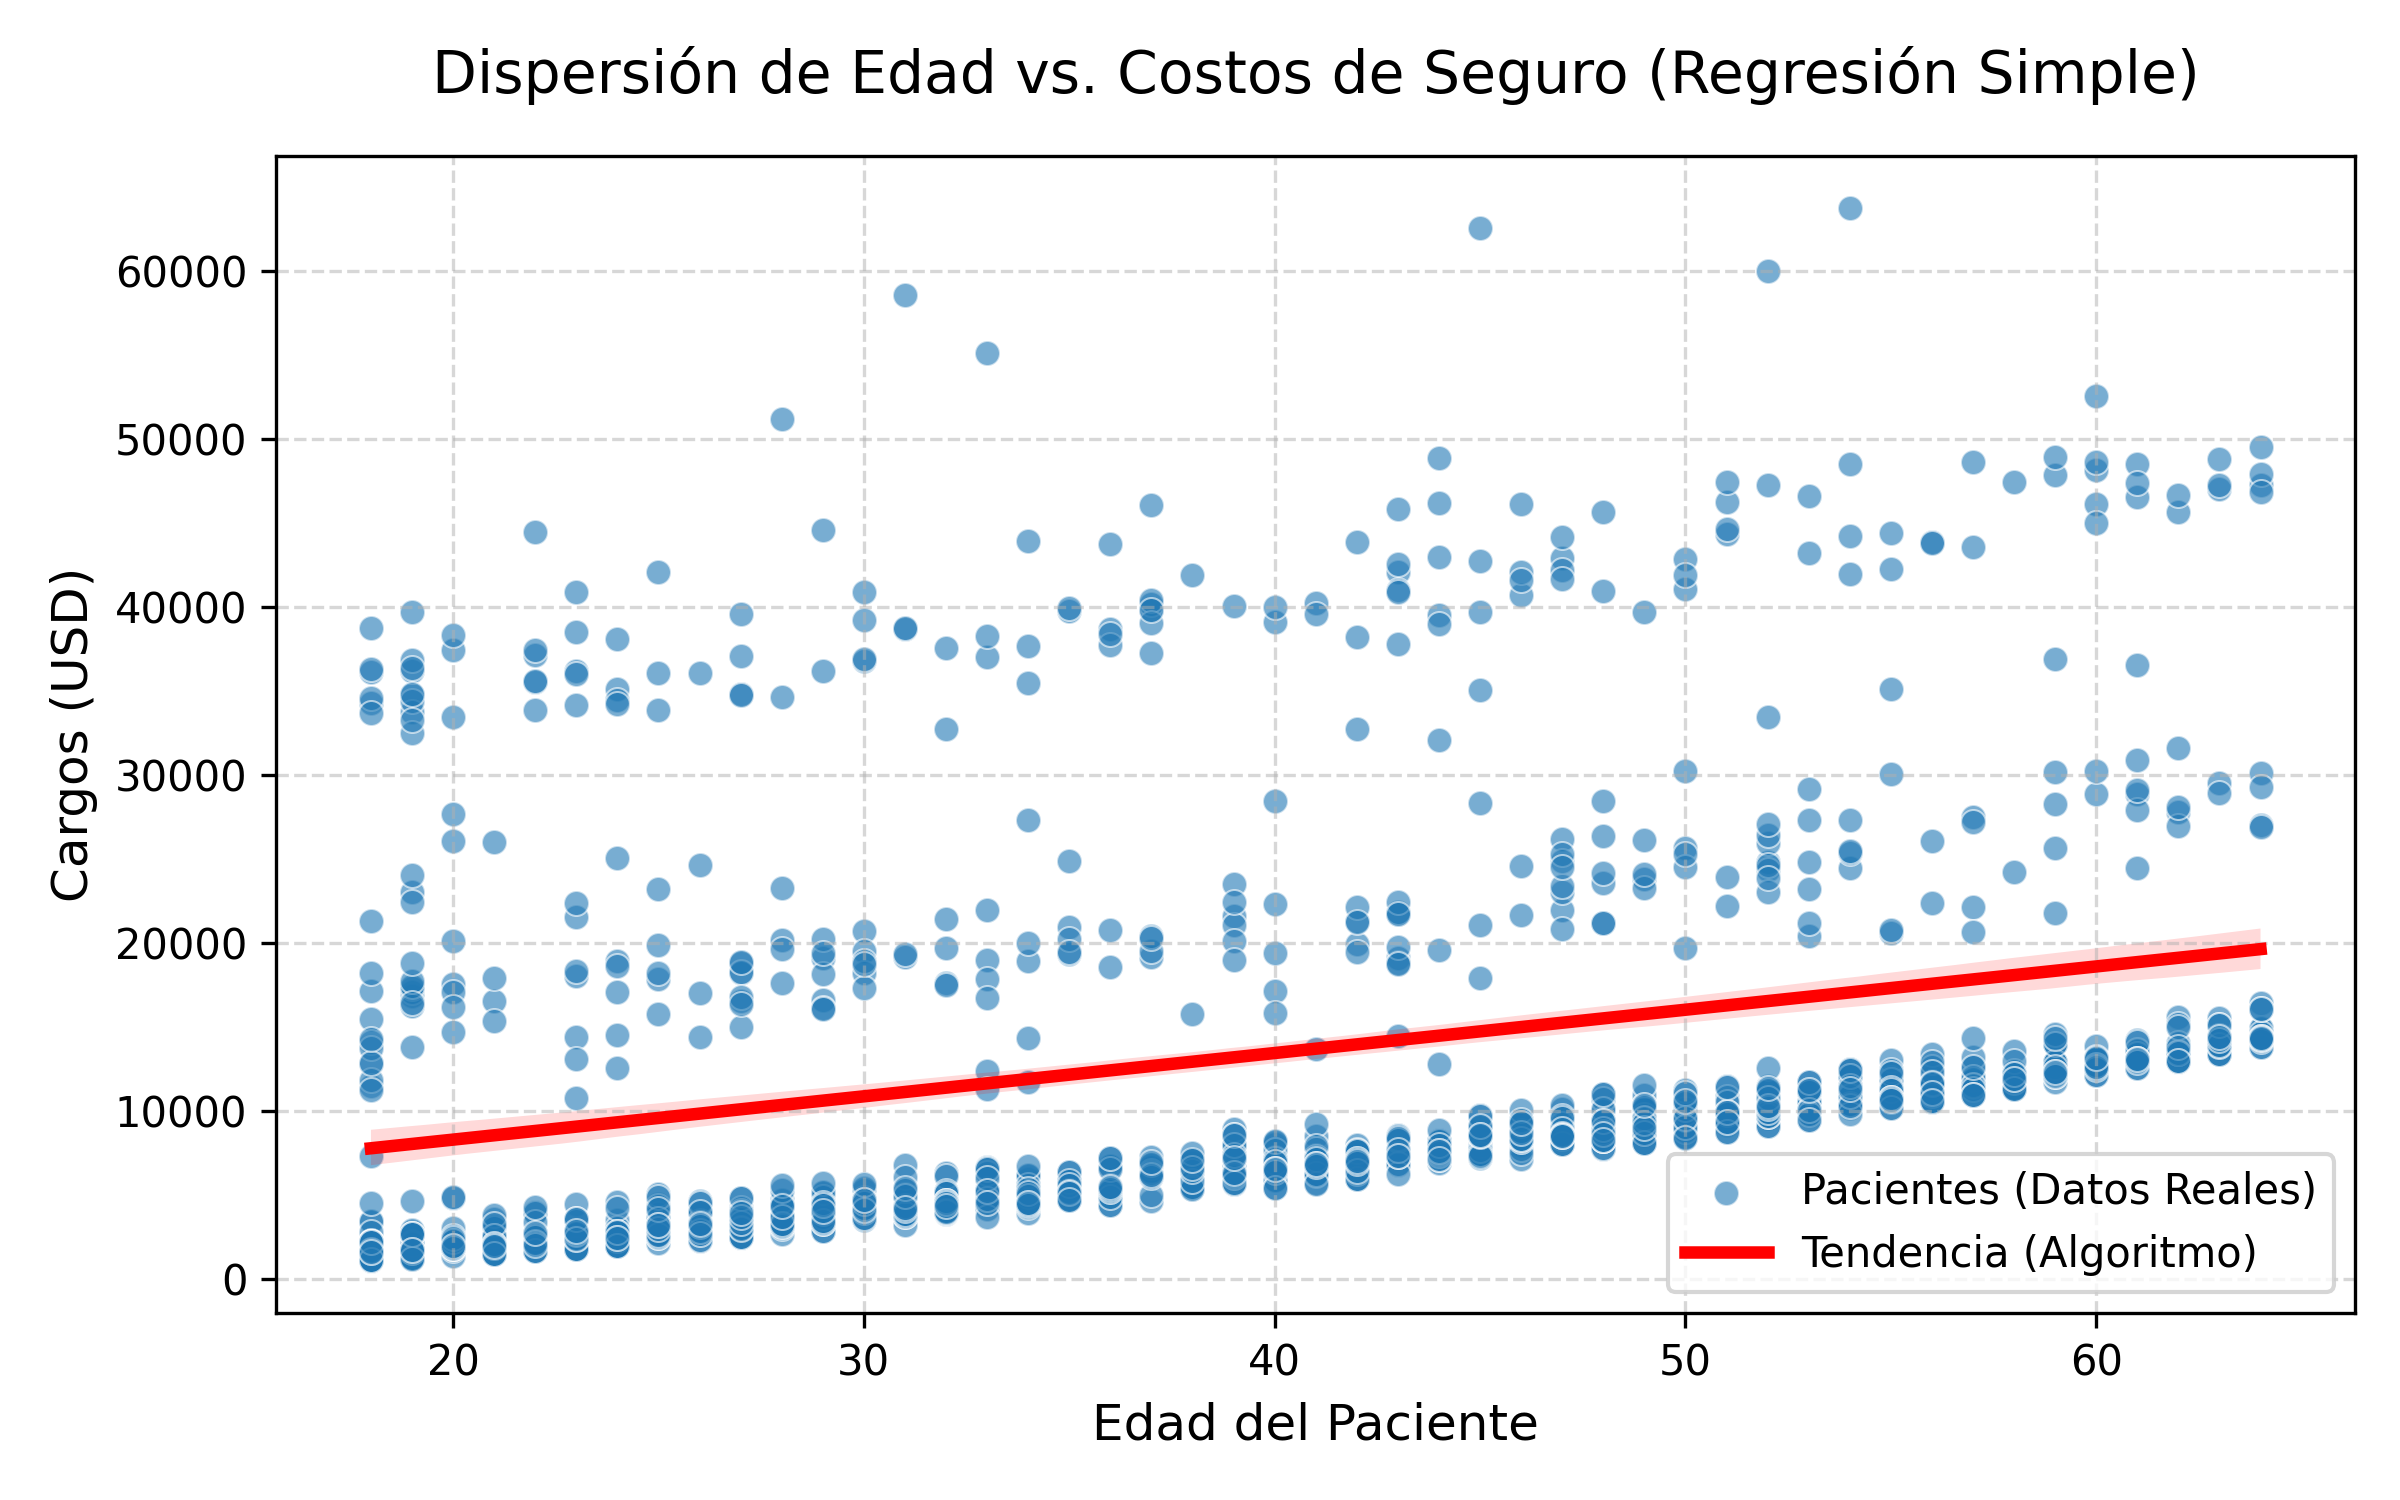
\includegraphics[width=0.6\textwidth]{grafica_simple.png}
\end{center}
\textbf{Interpretación:}
\begin{itemize}
    \item \textbf{Puntos Azules (Realidad):} Cada paciente real de nuestra base de datos.
    \item \textbf{Línea Roja (Tendencia):} El "estimador" matemático calculando la mejor trayectoria media.
    \item \textbf{Conclusión:} Al haber tanta dispersión alejada de la línea roja, deducimos empíricamente que un solo factor (Edad) no es suficiente.
\end{itemize}
\end{frame}

\begin{frame}[fragile]
\frametitle{Comandos Scikit-Learn: Regresión Simple (1/2)}
El flujo de trabajo en la librería \texttt{scikit-learn} consta de instanciar el modelo, ajustarlo a los datos (Entrenamiento) y generar predicciones.

\begin{block}{División de Entrenamiento y Prueba}
\begin{lstlisting}
from sklearn.model_selection import train_test_split

X = df_final[['age']] # Matriz 2D
y = df_final['charges'] # Vector 1D
X_train, X_test, y_train, y_test = train_test_split(X, y, test_size=0.20)
\end{lstlisting}
Separamos el $80\%$ de los datos para enseñar al modelo, y ocultamos el $20\%$ (\texttt{test}) para evaluar su precisión de forma imparcial.
\end{block}
\end{frame}

\begin{frame}[fragile]
\frametitle{Comandos Scikit-Learn: Regresión Simple (2/2)}

\begin{block}{Entrenamiento (Fit) y Predicción (Predict)}
\begin{lstlisting}
from sklearn.linear_model import LinearRegression

# 1. Crear el algoritmo
modelo_simple = LinearRegression()

# 2. Entrenar (El algoritmo calcula los betas)
modelo_simple.fit(X_train, y_train)

# 3. Predecir datos nuevos
predicciones = modelo_simple.predict(X_test)
\end{lstlisting}
El método \texttt{fit()} es donde ocurre el cálculo de Mínimos Cuadrados Ordinarios (OLS). El método \texttt{predict()} aplica la ecuación generada a nuevos datos.
\end{block}
\end{frame}

% -------------------------
% SECCIÓN 5: EVALUACIÓN
% -------------------------
\begin{frame}
\frametitle{Evaluación de Desempeño: ¿Es un buen modelo?}
Para auditar la validez del modelo, comparamos los valores reales (\texttt{y\_test}) contra nuestras proyecciones (\texttt{predicciones}).

\begin{itemize}
    \item \textbf{MAE (Error Absoluto Medio):} Promedio del error en la misma escala (ej. Dólares).
    \item \textbf{MSE (Error Cuadrático Medio):} Penaliza severamente los errores grandes elevándolos al cuadrado.
    \item \textbf{RMSE (Raíz del MSE):} Devuelve el MSE a la unidad original para su interpretación de negocio.
    \item \textbf{$R^2$ (Coeficiente de Determinación):} Representa el porcentaje (0.0 a 1.0) de la varianza en $y$ que es explicada por el modelo. Un valor de $0.80$ significa un modelo $80\%$ certero.
\end{itemize}
\end{frame}

\begin{frame}[fragile]
\frametitle{Comandos Scikit-Learn: Métricas}

\begin{block}{Extracción de Métricas de Evaluación}
\begin{lstlisting}
from sklearn.metrics import mean_squared_error, r2_score
import numpy as np

# R-Cuadrado (0.0 a 1.0)
r2 = r2_score(y_test, predicciones)

# RMSE (En dolares)
mse = mean_squared_error(y_test, predicciones)
rmse = np.sqrt(mse) 

print(f"R-Cuadrado: {r2}")
print(f"Error RMSE: {rmse}")
\end{lstlisting}
\end{block}
\end{frame}

% -------------------------
% SECCIÓN 6: REGRESIÓN MÚLTIPLE
% -------------------------
\begin{frame}
\frametitle{Regresión Lineal Múltiple: La Realidad Multidimensional}
Un solo factor (como la Edad) genera modelos imprecisos. La regresión \textbf{múltiple} incorpora varias variables, formando un "hiperplano" multidimensional:
\begin{center}
\Large $y = \beta_0 + \beta_1 X_1 + \beta_2 X_2 + \beta_3 X_3 + \dots$
\end{center}
\vspace{0.3cm}
\begin{itemize}
    \item $X_1$: Edad del paciente
    \item $X_2$: Índice de Masa Corporal (IMC)
    \item $X_3$: Estado de Fumador (0 = No, 1 = Sí)
\end{itemize}
\vspace{0.3cm}
El código de Scikit-Learn es \textbf{exactamente el mismo}. La única diferencia es que la matriz \texttt{X} contendrá múltiples columnas.
\end{frame}

\begin{frame}[fragile]
\frametitle{Escalado en la Regresión Múltiple}
Al tener múltiples variables, sus escalas numéricas varían (ej. Edades en decenas, pero salarios en miles). Debemos homogeneizarlas para que el algoritmo no asuma erróneamente que los números grandes son más importantes.

\begin{block}{StandardScaler}
\begin{lstlisting}
from sklearn.preprocessing import StandardScaler

scaler = StandardScaler()
X_mult[['age', 'bmi']] = scaler.fit_transform(X_mult[['age', 'bmi']])
\end{lstlisting}
El \texttt{StandardScaler} transforma las columnas continuas para que tengan media 0 y desviación estándar 1 (Z-Score).
\end{block}
\end{frame}

\begin{frame}
\frametitle{Guía Visual: Realidad vs. Predicción}
No podemos dibujar un hiperplano en 4D o 5D. Para evaluar un modelo múltiple, hacemos que compita contra la realidad:

\begin{center}
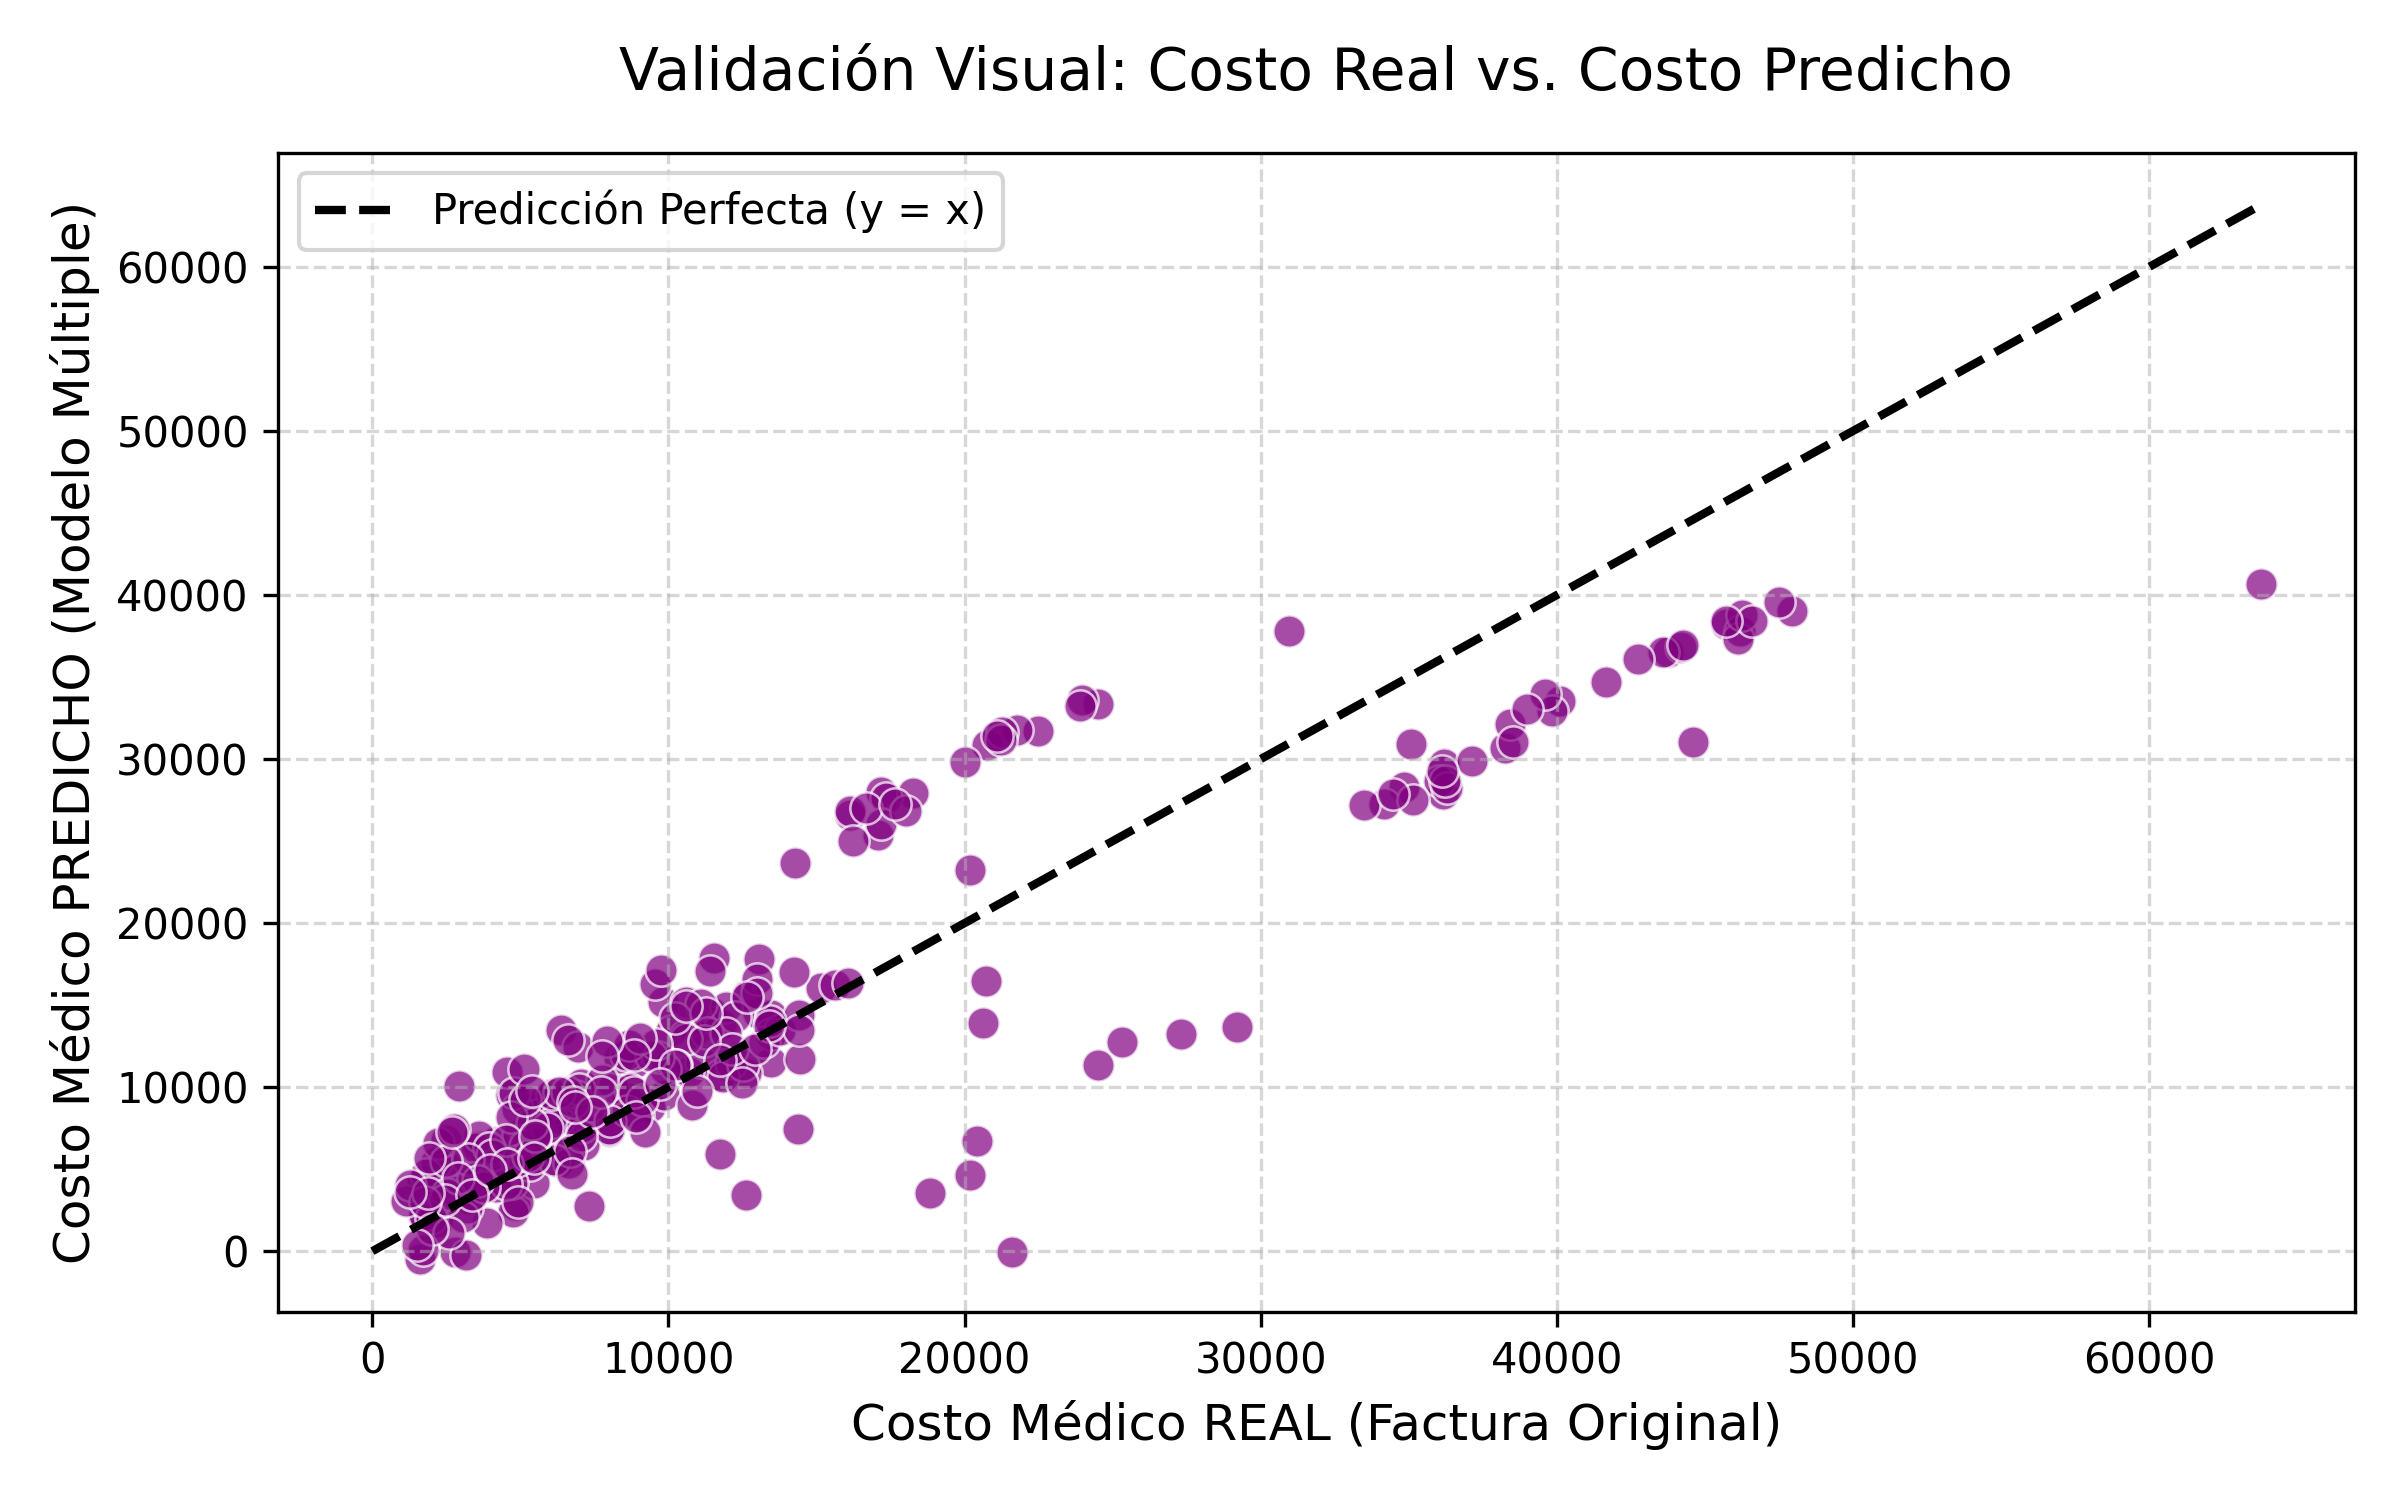
\includegraphics[width=0.55\textwidth]{grafica_multiple.png} 
\end{center}

\textbf{Interpretación:}
\begin{itemize}
    \item \textbf{Eje X:} Cargos Reales. \textbf{Eje Y:} Cargos Predichos.
    \item \textbf{Línea Negra (Diagonal):} La Perfección matemática ($y=x$).
    \item Si el modelo es preciso, los puntos morados abrazarán ajustadamente la línea diagonal.
\end{itemize}
\end{frame}

% -------------------------
% SECCIÓN 7: INFERENCIA DE NEGOCIO
% -------------------------
\begin{frame}[fragile]
\frametitle{Inferencia de Negocio: Interpretando los Coeficientes}
La Regresión Lineal destaca por su "transparencia". Podemos extraer los pesos algorítmicos ($\beta$) asociados a cada variable.

\begin{block}{Extracción de Coeficientes}
\begin{lstlisting}
# Imprimir coeficientes asignados a las variables
print(modelo_multiple.coef_)
\end{lstlisting}
\end{block}

\begin{table}
\centering
\begin{tabular}{lc}
\toprule
\textbf{Variable Evaluada} & \textbf{Impacto Económico Monetario ($\beta$)} \\
\midrule
Edad (Estandarizada) & $+\$3,500$ \\
IMC (Estandarizada) & $+\$2,000$ \\
\textbf{Fumador (\textit{smoker\_yes})} & $\mathbf{+\$23,800}$ \\
\bottomrule
\end{tabular}
\end{table}

\textbf{Análisis Analítico:} Si comparamos a dos pacientes idénticos en edad y peso físico, el riesgo de ser \textbf{Fumador} eleva el costo médico predicho en casi \$24,000 USD adicionales.
\end{frame}

\begin{frame}
\frametitle{Resumen de la Sesión}
\begin{itemize}
    \item \textbf{Preprocesamiento Crítico:} Transformar el texto (Fumador: Sí/No) a números (One-Hot Encoding) y escalar las magnitudes es un requisito ineludible.
    \item \textbf{Flujo Estándar:} Todo modelo en Python sigue la secuencia \texttt{Instanciar $\rightarrow$ fit() $\rightarrow$ predict()}.
    \item \textbf{Simple vs Múltiple:} Agregar dimensiones incrementa dramáticamente la exactitud predictiva (ej. El $R^2$ subió del 9\% al 76\%).
    \item \textbf{Inferencia:} Los algoritmos lineales permiten extraer reglas de negocio directas mediante sus coeficientes.
\end{itemize}
\end{frame}

\end{document}
